\begin{activity}{Stability, Time Stepping, and Information Transfer}

\section*{Purpose}
To develop physical intuition for numerical stability in explicit finite difference schemes.  In a time-stepping model, a field is updated step-by-step. Each step (iteration) uses information from neighboring nodes.  Think of information as spreading gradually through the system.

\section*{Learning Outcomes}

By the end of this activity, you should be able to:
\begin{itemize}
  \item State the stability condition for the explicit finite difference heat equation and identify the quantities it depends on.
  \item Explain physically why the allowable time step is proportional to $\Delta z^2$ and inversely proportional to $\kappa$.
  \item Describe what physically happens when the stability limit is exceeded, and why this corresponds to physically impossible behavior.
  \item Compare stability requirements for materials with different thermal diffusivities.
\end{itemize}
}

\section*{Part A: Prediction and reasoning}
Before running anything, discuss:
\begin{itemize}
    \item What do you expect for a very small time step? A very large one?
    \item Heat diffuses at a rate set by $\kappa$. Why can't it move arbitrarily far
    in a single time step?
\end{itemize}
\answerbox[3cm]

\section*{Part A: What breaks, and when}
Your instructor will run the explicit finite-difference solver for the diffusion
equation ($\kappa = 1$) at several time steps $\Delta t$, holding $\Delta z$ fixed.
Record what you observe for each run (smooth decay, mild wobble, or blow-up), then
compute $\Delta t / \Delta z^2$ for each case.
\answerbox[3.5cm]

\textbf{Task:} Looking at your table, what value of $\Delta t/\Delta z^2$ seems to
separate stable runs from unstable ones?
\answerbox[2cm]

\section*{Part B: Reading the stability condition}
For a one-dimensional explicit scheme,
\[
\Delta t < \frac{\Delta z^2}{2\kappa}.
\]
Compare this to the threshold you found in Part A. \textbf{Explain} why the allowable
time step depends on $\Delta z$ and $\kappa$ the way it does --- what does this mean
physically, in terms of how far thermal information can travel between nodes in one
step?
\answerbox[4cm]

\textit{Optional --- if time permits:} Your instructor also ran the implicit and
Crank--Nicolson schemes at the same unstable $\Delta t$. Both stayed stable. If implicit
methods are unconditionally stable, why would anyone still use the explicit scheme?

\section*{Part B: Physical reasoning}

Interpret the stability condition as a limit on how fast thermal information can move between nodes.

Why can heat not ``jump'' over nodes in a single time step?

What determines how quickly heat diffuses through a material?
\answerbox[3cm]

\bigskip

{\color{red}
\section*{Key Ideas}

Numerical instability occurs when the model allows heat to propagate faster than physically possible.

{\color{blue}
\textbf{The stability condition is a physical causality constraint.} Heat diffuses at a rate set by $\kappa$. In a time step $\Delta t$, physical heat can travel at most $\sqrt{\kappa\,\Delta t}$. The stability condition $\Delta t < \Delta z^2/2\kappa$ ensures that this thermal length cannot exceed the node spacing $\Delta z$. Violating the condition means asking the model to move heat further in one step than the physics allows.

\begin{figure}[h]
\centering
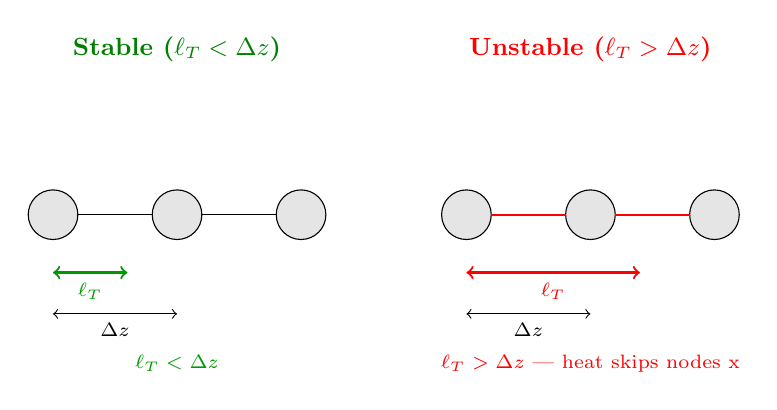
\begin{tikzpicture}[scale=1.05]
  % --- Stable case ---
  \node[font=\small\bfseries, green!50!black] at (1.5, 2.0) {Stable ($\ell_T < \Delta z$)};
  \foreach \x in {0, 1.5, 3.0} {
    \draw[fill=gray!20] (\x, 0) circle (0.3);
  }
  \draw (0.3,0) -- (1.2,0);
  \draw (1.8,0) -- (2.7,0);
  \draw[<->, thick, green!60!black] (0,-0.7) -- (0.9,-0.7)
    node[midway, below, font=\scriptsize] {$\ell_T$};
  \draw[<->] (0,-1.2) -- (1.5,-1.2)
    node[midway, below, font=\scriptsize] {$\Delta z$};
  \node[font=\scriptsize, green!60!black] at (1.5,-1.8) {$\ell_T < \Delta z$ \checkmark};

  % --- Unstable case ---
  \node[font=\small\bfseries, red] at (6.5, 2.0) {Unstable ($\ell_T > \Delta z$)};
  \foreach \x in {5.0, 6.5, 8.0} {
    \draw[fill=gray!20] (\x, 0) circle (0.3);
  }
  \draw[red, thick] (5.3,0) -- (6.2,0);
  \draw[red, thick] (6.8,0) -- (7.7,0);
  \draw[<->, thick, red] (5.0,-0.7) -- (7.1,-0.7)
    node[midway, below, font=\scriptsize] {$\ell_T$};
  \draw[<->] (5.0,-1.2) -- (6.5,-1.2)
    node[midway, below, font=\scriptsize] {$\Delta z$};
  \node[font=\scriptsize, red] at (6.5,-1.8) {$\ell_T > \Delta z$ — heat skips nodes x};
\end{tikzpicture}
\caption{Stability requires that the thermal length $\ell_T = \sqrt{\kappa\,\Delta t}$ does not exceed the node spacing $\Delta z$. When it does, heat is asked to propagate past neighboring nodes in one step, which is physically impossible and causes numerical blow-up.}
\end{figure}
}

\textbf{Finer grids require smaller time steps.} Because stability scales as $\Delta z^2$, halving the grid spacing reduces the maximum allowable time step by a factor of four. Increasing resolution is therefore expensive: the number of spatial nodes doubles \emph{and} the number of time steps quadruples to cover the same total time.

\textbf{High diffusivity is more demanding numerically.} Materials with large $\kappa$ (e.g., peridotite, ice) diffuse heat quickly and require smaller time steps for numerical stability than low-diffusivity materials (e.g., clay-rich sediments). This is the reverse of the geological situation: fast-diffusing materials are easier to model geologically but harder numerically.
}

\end{activity}